% This file was created by tikzplotlib v0.9.1.
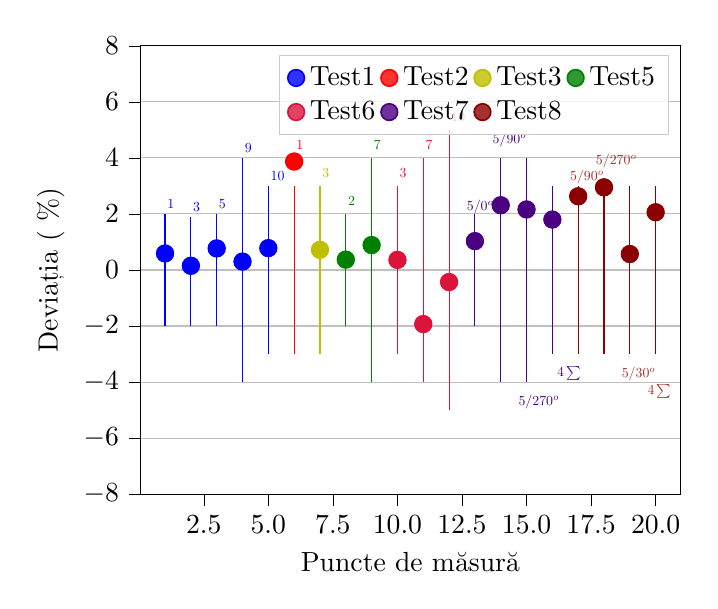
\begin{tikzpicture}

\definecolor{color0}{rgb}{0.75,0.75,0}
\definecolor{color1}{rgb}{0.862745098039216,0.0784313725490196,0.235294117647059}
\definecolor{color2}{rgb}{0.294117647058824,0,0.509803921568627}
\definecolor{color3}{rgb}{0.647058823529412,0.164705882352941,0.164705882352941}

\begin{axis}[
legend cell align={left},
legend columns=4,
legend style={fill opacity=0.8, draw opacity=1, text opacity=1, draw=white!80!black},
tick align=outside,
tick pos=left,
x grid style={white!69.0196078431373!black},
xlabel={Puncte de măsură},
xmin=0.0499999999999999, xmax=20.95,
xtick style={color=black},
xtick={0,2.5,5,7.5,10,12.5,15,17.5,20,22.5},
xticklabels={\(\displaystyle 0.0\),\(\displaystyle 2.5\),\(\displaystyle 5.0\),\(\displaystyle 7.5\),\(\displaystyle 10.0\),\(\displaystyle 12.5\),\(\displaystyle 15.0\),\(\displaystyle 17.5\),\(\displaystyle 20.0\),\(\displaystyle 22.5\)},
y grid style={white!75.2941176470588!black},
ylabel={Deviația ( \(\displaystyle \%\))},
ymajorgrids,
ymin=-8, ymax=8,
ytick style={color=black},
ytick={-8,-6,-4,-2,0,2,4,6,8},
yticklabels={\(\displaystyle -8\),\(\displaystyle -6\),\(\displaystyle -4\),\(\displaystyle -2\),\(\displaystyle 0\),\(\displaystyle 2\),\(\displaystyle 4\),\(\displaystyle 6\),\(\displaystyle 8\)}
]
\path [draw=blue]
(axis cs:1,-2)
--(axis cs:1,2);

\path [draw=blue]
(axis cs:2,-2)
--(axis cs:2,1.9);

\path [draw=blue]
(axis cs:3,-2)
--(axis cs:3,2);

\path [draw=blue]
(axis cs:4,-4)
--(axis cs:4,4);

\path [draw=blue]
(axis cs:5,-3)
--(axis cs:5,2.98);

\path [draw=red]
(axis cs:6,-3)
--(axis cs:6,3);

\path [draw=color0]
(axis cs:7,-3)
--(axis cs:7,3);

\path [draw=green!50!black]
(axis cs:8,-2)
--(axis cs:8,2);

\path [draw=green!50!black]
(axis cs:9,-4)
--(axis cs:9,4);

\path [draw=color1]
(axis cs:10,-3)
--(axis cs:10,3);

\path [draw=color1]
(axis cs:11,-4)
--(axis cs:11,4);

\path [draw=color1]
(axis cs:12,-5)
--(axis cs:12,5);

\path [draw=color2]
(axis cs:13,-2)
--(axis cs:13,2);

\path [draw=color2]
(axis cs:14,-4)
--(axis cs:14,4);

\path [draw=color2]
(axis cs:15,-4)
--(axis cs:15,4);

\path [draw=color2]
(axis cs:16,-3)
--(axis cs:16,3);

\path [draw=red!54.5098039215686!black]
(axis cs:17,-3)
--(axis cs:17,3);

\path [draw=red!54.5098039215686!black]
(axis cs:18,-3)
--(axis cs:18,3);

\path [draw=red!54.5098039215686!black]
(axis cs:19,-3)
--(axis cs:19,3);

\path [draw=red!54.5098039215686!black]
(axis cs:20,-3)
--(axis cs:20,3);

\addplot [semithick, blue, mark=*, mark size=3, mark options={solid}, only marks]
table {%
1 0.59
2 0.15
3 0.77
4 0.3
5 0.78
};
\addlegendentry{Test1}
\addplot [semithick, red, mark=*, mark size=3, mark options={solid}, only marks]
table {%
6 3.87
};
\addlegendentry{Test2}
\addplot [semithick, color0, mark=*, mark size=3, mark options={solid}, only marks]
table {%
7 0.72
};
\addlegendentry{Test3}
\addplot [semithick, green!50!black, mark=*, mark size=3, mark options={solid}, only marks]
table {%
8 0.37
9 0.89
};
\addlegendentry{Test5}
\addplot [semithick, color1, mark=*, mark size=3, mark options={solid}, only marks]
table {%
10 0.36
11 -1.93
12 -0.43
};
\addlegendentry{Test6}
\addplot [semithick, color2, mark=*, mark size=3, mark options={solid}, only marks]
table {%
13 1.03
14 2.31
15 2.16
16 1.8
};
\addlegendentry{Test7}
\addplot [semithick, red!54.5098039215686!black, mark=*, mark size=3, mark options={solid}, only marks]
table {%
17 2.63
18 2.95
19 0.57
20 2.06
};
\addlegendentry{Test8}
\addplot [blue, mark=*, mark size=3, mark options={solid}, only marks, forget plot]
table {%
1 0.59
2 0.15
3 0.77
4 0.3
5 0.78
};
\addplot [red, mark=*, mark size=3, mark options={solid}, only marks, forget plot]
table {%
6 3.87
};
\addplot [color0, mark=*, mark size=3, mark options={solid}, only marks, forget plot]
table {%
7 0.72
};
\addplot [green!50!black, mark=*, mark size=3, mark options={solid}, only marks, forget plot]
table {%
8 0.37
9 0.89
};
\addplot [color1, mark=*, mark size=3, mark options={solid}, only marks, forget plot]
table {%
10 0.36
11 -1.93
12 -0.43
};
\addplot [color2, mark=*, mark size=3, mark options={solid}, only marks, forget plot]
table {%
13 1.03
14 2.31
15 2.16
16 1.8
};
\addplot [red!54.5098039215686!black, mark=*, mark size=3, mark options={solid}, only marks, forget plot]
table {%
17 2.63
18 2.95
19 0.57
20 2.06
};
\draw (axis cs:0.9,2.2) node[
  scale=0.5,
  anchor=base west,
  text=blue,
  rotate=0.0
]{1};
\draw (axis cs:1.9,2.1) node[
  scale=0.5,
  anchor=base west,
  text=blue,
  rotate=0.0
]{3};
\draw (axis cs:2.9,2.2) node[
  scale=0.5,
  anchor=base west,
  text=blue,
  rotate=0.0
]{5};
\draw (axis cs:3.9,4.2) node[
  scale=0.5,
  anchor=base west,
  text=blue,
  rotate=0.0
]{9};
\draw (axis cs:4.9,3.18) node[
  scale=0.5,
  anchor=base west,
  text=blue,
  rotate=0.0
]{10};
\draw (axis cs:5.9,4.3) node[
  scale=0.5,
  anchor=base west,
  text=red,
  rotate=0.0
]{1};
\draw (axis cs:6.9,3.3) node[
  scale=0.5,
  anchor=base west,
  text=color0,
  rotate=0.0
]{3};
\draw (axis cs:7.9,2.3) node[
  scale=0.5,
  anchor=base west,
  text=green!50!black,
  rotate=0.0
]{2};
\draw (axis cs:8.9,4.3) node[
  scale=0.5,
  anchor=base west,
  text=green!50!black,
  rotate=0.0
]{7};
\draw (axis cs:9.9,3.3) node[
  scale=0.5,
  anchor=base west,
  text=color1,
  rotate=0.0
]{3};
\draw (axis cs:10.9,4.3) node[
  scale=0.5,
  anchor=base west,
  text=color1,
  rotate=0.0
]{7};
\draw (axis cs:11.9,5.3) node[
  scale=0.5,
  anchor=base west,
  text=color1,
  rotate=0.0
]{10};
\draw (axis cs:12.5,2.12) node[
  scale=0.5,
  anchor=base west,
  text=color2,
  rotate=0.0
]{$5/0^o$};
\draw (axis cs:13.5,4.52) node[
  scale=0.5,
  anchor=base west,
  text=color2,
  rotate=0.0
]{$5/90^o$};
\draw (axis cs:14.5,-4.84) node[
  scale=0.5,
  anchor=base west,
  text=color2,
  rotate=0.0
]{$5/270^o$};
\draw (axis cs:16,-3.8) node[
  scale=0.5,
  anchor=base west,
  text=color2,
  rotate=0.0
]{$4\sum$};
\draw (axis cs:16.5,3.18) node[
  scale=0.5,
  anchor=base west,
  text=color3,
  rotate=0.0
]{$5/90^o$};
\draw (axis cs:17.5,3.78) node[
  scale=0.5,
  anchor=base west,
  text=color3,
  rotate=0.0
]{$5/270^o$};
\draw (axis cs:18.5,-3.84) node[
  scale=0.5,
  anchor=base west,
  text=color3,
  rotate=0.0
]{$5/30^o$};
\draw (axis cs:19.5,-4.44) node[
  scale=0.5,
  anchor=base west,
  text=color3,
  rotate=0.0
]{$4\sum$};
\end{axis}

\end{tikzpicture}
